\chapter{Sugestões Proto-históricas}\label{app:B}

Descrevemos neste capítulo um trabalho de \citeonline{mathews_groove_1970}, GROOVE, ainda pouco observado por improvisadores de códigos e a atuação de uma tecnologia, a compilação JIT \cite{aycock_brief_2003} como um sujeito sócio-técnico fundamental para que o \emph{live coding} fosse possível.

\section{GROOVE}

GROOVE, ou \emph{Generated Real-time Operations On Voltage-controlled Equipment} foi um computador desenvolvido na Bell Labs por \cite{mathews_groove_1970}. Alex \citeonline{di_nunzio_genesi_2010} discute como um precedente direto do família de \emph{softwares} MUSIC N\footnote{Desenvolvidos a partir de 1957. As versões \emph{softwares} MUSIC I, II, III, IV, IV-B, IV-BF, V (que passou por modificações no IRCAM), MUSIC 360, MUSIC 11 acarretaram no desenvolvimento do \emph{software} CSound, disponível em \url{https://csound.github.io/}.}. É o primeiro de trabalho de Mathews com reflexões nos aspectos performáticos. Não foi usado para ambientes de performance, mas a peça \emph{The expanding universe} da compositora Laurie \citeonline{spiegel_expanding_1975} foi considerada como exemplar por sua execução instrumental e disponibilidade \emph{online} (ver a seguir). Seu desenvolvimento iniciou em 1968 na \emph{Bell Labs}. Segundo o próprio Mathews, o funcionamento do sistema oferece algumas possibilidades a partir de três conceitos: \emph{criação}, \emph{retroalimentação} e \emph{ciberficação}. O primeiro conceito foi implementado com um sistema de arquivos, onde as funções criadas no processo criativo são memorizadas, e podem ser editadas. O segundo conceito se relaciona com o terceiro:

\traduzcitacao{
O GROOVE provê oportunidades para uma retroalimentação imediata de observações dos efeitos das funções temporais para as entradas do computador, que compõem a função. No modo de composição do sistema GROOVE, um ser humano está em um ciclo de retroalimentação, como mostrado na figura 1 $[$\autoref{fig:groove_sistema}$]$. Assim ele é capaz de modificar as funções instantâneamente como um resultado de suas observações daqueles efeitos
}
{
GROOVE provides opportunity for immediate feedback from observations of the effects of time functions to computer inputs which compose the function. In the compose mode of the GROOVE system, a human beign is in the feedback loop (\ldots) Thus he is able to modify the functions instanteneously as a result of his observations of their effects.
}
{p.~715}{mathews_groove_1970}

\begin{figure}
\begin{center}
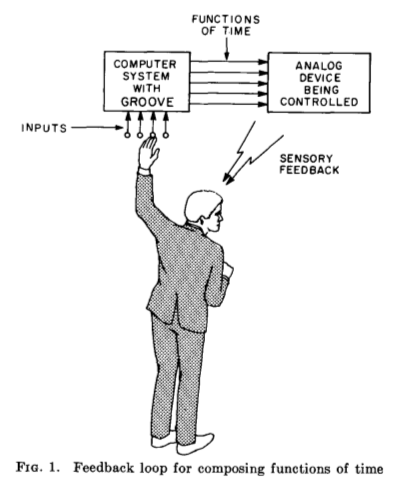
\includegraphics[scale=0.618]{./imagens/GROOVE.png}
\caption{Esquema de concepção do projeto GROOVE. \textbf{Fonte}: \cite{mathews_groove_1970}.}
\label{fig:groove_sistema}
\end{center}
\end{figure} 

O terceiro conceito observa a existência de uma relação entre um humano e uma máquina. Mathews descreve-o como uma \emph{engenharia humana}. Esta engenharia consistiu na observação de um tempo diferencial entre o que o(a) musicista cria e o que edita:

\traduzcitacao{
O conceito final é mais nebuloso. Desde que o GROOVE é um sistema homem-máquina, a engenharia humana do sistema foi a mais importante. Por exemplo, nós descobrimos que o controle do programa de tempo necessita ser bastante diferente para a composição do que para a edição, e o programa foi modificado de acordo. (\ldots) O intérprete de computador não deve tentar definir todo o som em tempo real. Ao invés, o computador deve ter uma partitura e o intérprete deve influenciar a forma como a partitura é tocada. Seus modos de influência podem ser mais variados do que aqueles que um regente convencional, que pode principalmente controloar o tempo, intensidade, e estilo
}
{
The final concept is more nebulous. Since GROOVE is a man-computer system, the human engeneering of the system is most important. For example, we discovered that the control of the program time needs to be quite different for composing than for editing, and the program was modiffied accordingly. (\ldots) The computer performer should not attempt to define the entire sound in real-time. Instead, the computer should have a score and the performer should influence the way in which the score is played. His modes of influence can be much more varied than that a conventional conductor who primarily controls tempo, loudness, and style.
}
{p.~715-716}{mathews_groove_1970}


Como exemplo , selecionamos uma descrição da compositora Laurie \citeonline{spiegel_expanding_1975} (ver \autoref{fig:groove}) para sumarizar as características do GROOVE, durante a produção de \emph{The Expanding Universe} \footnote{Disponível em \url{https://www.youtube.com/watch?v=dYUZmsfm4Ww}.}, entre as salas 2D-506 da Bell Labs (contendo o computador DDP-224) e a sala analógica 2D-562 (laboratório de Mathews). A ``performance'' da obra era realizada, com a programação de funções temporais e a manipulação de parâmetros dessas funções através de dispositivos físicos:

\begin{citacao}
Todas as músicas no GROOVE eram representadas na memória digital como funções abstratas do tempo, séries paralelas de dois pontos, cada ponto sendo um instante no tempo e um valor instantâneo. A taxa de amostragem para essas funções, usada principalmente como controle de voltagem, era cronometrada por um grande e antiquado oscilador analógico que era normalmente fixado em 100 Hertz, cada ciclo do oscilador pulsando à frente do código, o computador lia, em cada uma das funções, naquele ponto do tempo, todos dispositivos de entrada e executava todas amostras. (\ldots) Tínhamos uma pequena caixa com 4 potenciômetros e quatro chaves (alternadores fixados onde você os colocava) e dois botões de disparo.\footnote{Tradução de \emph{All music in GROOVE was represented in digital memory as abstract functions of time, parallel series of point pairs, each point being an instant in time and an instantaneous value. The sampling rate for these functions, which would be used mostly as control voltages, was clocked by a big old-fashioned analog oscillator that was usually set to 100 Hertz, each cycle of the oscillator pulsing one run through the code, the computer reading all of the real time input devices and playing of all of the samples at that time point in each of the time functions. (\ldots)  We had a small box with 4 knobs, 4 set switches (toggles that stay where you put them) and 2 momentary-contact push buttons on it.}}
\end{citacao}

\begin{figure}[!h]
  \begin{center}
  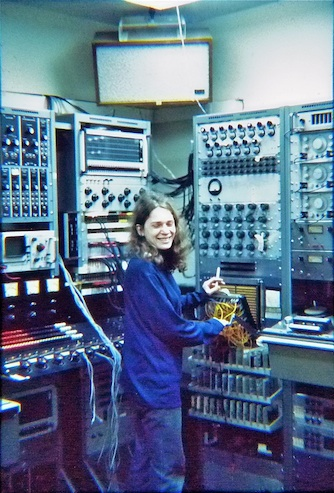
\includegraphics[scale=0.618]{./imagens/spiegel.jpg}
  \caption{\small Laurie Spiegel configurando a saída analógica do GROOVE, durante a produção de \emph{The Expanding Universe}. \textbf{Fonte}: \cite{spiegel_expanding_1975}.}
  \label{fig:groove}
  \end{center}
\end{figure}

Embora não declare ser uma peça minimalista, a descrição de \emph{The Expanding Universe} considera, de maneira asséptica, os fenômenos psicoacústicos como elementos composicionais. Por exemplo, a utilização da continuidade progressiva de sons (ou \emph{drones} transitórios) como elemento criativo permite, segundo a compositora, à sensibilização do ouvido, o que não seria possível na música minimalista instrumental:

\begin{citacao}
 A violência da perturbação sonora, disjunção, descontinuidade e mudanças súbitas desanitizam o ouvinte e nos afastam, de forma que não estamos mais abertos aos sons mais sutis. Mas com continuidade e gentileza, o ouvido se torna re-sensibilizado para mais e mais fenômenos auditoriais sutis dentro do som que estamos imersos. Em vez de sermos arrastados, como nas cascatas de muitas notas executadas em blocos de tempo que mudam repentinamente, tal como tantas vezes consite a música "minimalista", abrimos nossos ouvidos mais e mais para os fenômenos que nos envolvem. Isto também não é música ambiente, um termo que veio a ser usado alguns anos depois. Esta é música para atenção concentrada, uma experiência musical do através, pensando que, lógico, existe também um pano de fundo. \footnote{Tradução de\emph{The violence of sonic disruption, disjunction, discontinuity and sudden change desensitizes the listener and pushes us away so we are no longer open to the subtlest sounds. But with continuity and gentleness, the ear becomes increasingly re-sensitized to more and more subtle auditory phenomena within the sound that immerses us. Instead of being swept along, as with cascades of many running notes in suddenly-changing blocks of time, such as “minimalist” music so often consists of, we open up our ears more and more to the more minute phenomena that envelope us. This is also not “ambient music”, a term that came into use some years later. This is music for concentrated attention, a through-composed musical experience, though of course it also can be background.}}
\end{citacao}

Nesta citação podemos sumarizar um conceito para o \emph{live coding}: Música como um Processo Gradual \cfcite{reich_music_1968}. Porém, o significado de processo pode ser desenvolvido infinitamente. Isso não será realizado. O Processo para Spiegel é diverso daquele considerado no \emph{live coding}, e uma digressão desta pode afastar demais o foco do trabalho principal. Para compreesão deste termo, será necessário explorar outros aspectos correlacionados no decorrer deste trabalho.

Para finalizar esta sessão, a figura \autoref{fig:groove} sugere um conceito rotineiro para o \emph{live coder}. Esta rotina é uma atividade constante de improvisação códigos para aquisição de destreza para uma performance. \citeonline{iazzetta_musica_2009,soares_luteria_2015} lembram que esta atividade, de codificar como se construísse um instrumento musical, se caracteriza por sua conexão com a esfera composicional, nomeado \emph{luteria composicional}.

\section{SuperCollider}

O SuperCollider\disponivelem{https://supercollider.github.io/} é um ambiente de programação desenvolvido por James McCartney, lançado em 1996. Segundo \citeonline{mccartney_supercollider_1996}, 

\begin{citacao}
\traducao{SuperCollider começou como dois programas separados que eu escrevi. O primeiro foi um programa chamado \emph{Synth-O-Matic} que era um sintetizador de tempo diferido, escrito de forma semelhante à linguagem C, para Machintosh em 1990 e foi abandonado. O segundo era um objeto \emph{MAX} chamado \emph{Pyrite} que continha um interpretador para a linguagem que se extendeu e foi usado no SuperCollider. Escrever o SuperCollider envolveu integrar uma linguagem interpretada, um coletor delixo $[$administração automática da memória$]$, e uma biblioteca de funções do Pyrite com uma máquina de síntese e funções do Synth-O-Matic. Eu gostaria de agradecer ao Curtis Roads por encorajar-me a reviver o programa do Synth-O-Matic, que levou ao SuperCollider.}{SuperCollider began as two separate programs that I wrote. The first was a program called Synth-O-Matic which was a non-real-time C-like synthesis programming language for the Macintosh written in 1990 and abandoned. The second was a MAX object called Pyrite which contained the interpreter for the language which was extended and used in SuperCollider. Writing SuperCollider involved integrating the language interpreter, garbage collector and function library of Pyrite with the synthesis engine and functions of Synth-O-Matic. I'd like to thank Curtis Roads for encouraging me to revive the Synth-O-Matic program which ultimately led to SuperCollider.}
\end{citacao}

Uma outra perspectiva é oferecida como uma possibilidade lógica e enxuta de outros paradigmas de programação musical.\citeonline[p.~1]{mccartney_supercollider_1996}, descreve alguns problemas com o paradigma de programação musical desenvolvido a partir do Music N \cite{mathews_digital_1963}, como por exemplo, a uma estrutura estática inerente à concepção de objetos conectados por cabos:

\begin{citacao}
\traducao{As abstrações fornecidas pelas linguagens MUSIC N, incluindo o CSound, são abstrações de unidades geradoras, o laço de computação para a amostra de áudio, a representação de conexões entre unidades geradoras, e instanciamento e desalocação de instrumentos. Estas abstrações tornaram a escrita de algoritmos de processamento de sinais mais fácil, porquê eles abstraem um número de detalhes incômodos. Contudo, a família Music N provê poucas estruturas de controle, nenhuma estrutura de dados reais, e nenhuma função de usuário. SAOL melhora o paradigma do Music N provendo tipos de abstrações encontradas na linguagem C, tais como estruturas de controle, funções e algumas estruturas de dados. Max, que é um tipo diferente de linguagem de programação, provê um conjunto interessante de abstrações que permite muitas pessoas usá-lo sem perceberem que estão programando acima de tudo. (\ldots) A linguagem Max també é limitada em sua habilidade de tratar seus objetos como dados, o que torna uma estrutura de objetos estáticos. Evoluções posteriores do Max, como o jMax, e o Pd, fazem várias coisas para expandir as limitações de estrutura de dados do Max, mas ainda assim possuem uma estrutura estática de objeto.
}
{
The abstractions provided by the Music N languages, including Csound (www.csounds.com), are the abstraction of a unit generator, the audio sample computation loop, the representation of the connections between unit generators, and instrument instantiation and de-allocation. These abstractions make writing signal-processing algorithms easier, because they abstract a number of cumbersome details. However, the Music N family provides few control structures, no real data structures, and no user functions. SAOL (www.saol.net) improves the Music N paradigm by providing the kinds of abstractions found in the C language, such as control structures, functions, and some data structures. Max (www.cycling74.com/products/maxmsp.html), which is quite a different kind of programming language, provides an interesting set of abstractions that enable many people to use it
without realizing they are programming at all. (\ldots). The Max language is also limited in its ability to treat its own objects as data, which makes for a static object structure. Later evolutions of Max, such as jMax (www.ircam.fr/produits/logiciels/log-forum/jmax-e.html) and Pd (www.pure-data.org), do various things to expand the data structure limitations of Max but still have a generally static object structure.
}
\end{citacao}

McCartney discute adiante um modelo alternativo de notação musical, adaptado aos padrões de uma linguagem que expresse comportamentos musicais, ao invés da determinação de pontos fixos de parâmetros musicais:

\begin{citacao}
\traducao{Uma lingagem musical de computador deve prover um conjunto de abstralções que expressam idéias composicionais e de processamento de sinais da maneira mais fácil e direta possível. Os tipos de idéias que alguém pode expressar, contudo, podem ser diferentes e levar para diferentes ferramentas. Se alguém interessado em realizar uma partitura que represente uma peça musical como um artefato fixado, então o modelo de partitura/orquestra será suficiente. Motivações que levaram a projetar o SuperCollider estavam na habilidade de perceber processos sonoros que são diferentes, a cada vez que eles são tocados, para escrever peças que de alguma forma descrevem um campo de possibilidades ao invés de uma entidade fixa, e o que facilita a improvisação ao vivo por um compositor/executante.}{
{A computer music language should provide a set of abstractions that makes expressing compositional and signal processing ideas as easy and direct as possible. The kinds of ideas one wishes to express, however, can be quite different and lead to very different tools. If one is interested in realizing a score that represents a piece of music as a fixed artifact, then a traditional orchestra/score model will suffice. Motivations for the design of SuperCollider were the ability to realize sound processes that were different every time they are played, to write pieces in a way that describes a range of possibilities rather than a fixed entity, and to facilitate live improvisation by a composer/performer.
}
\end{citacao}

Um exemplo de uso pode ilustrar o discurso do McCartney. O exemplo abaixo (p.~\pageref{ex:artificial}) é um código de Fredrik Olofson, outro personagem importante para a improvisação de códigos \cite{ward_live_2004}. Este exemplo é peculiar, uma vez que expõe não somente estruturas dinâmicas e deterministas, mas possibilita criar uma conexão com dois assuntos discutidos anteriormente, algoraves \ver{sec:algorave} e microchips \ver{sec:baiadesaofransisco} .  Um sintetizador recria o timbre do videogame \emph{Atari2600} (laçado no EUA em 1977); mais especificamente é um simulador do \emph{chip} TIA (\emph{Television Interface Adapter}), responsável pela geração de gráficos e imagens no videogame Atari\disponivelem{https://www.atariage.com/2600/archives/schematics_tia/index.html}. O exemplo é relativamente simples. Um sintetizador (\verb|SynthDef|) e um sequenciador (\verb|Pbind|)são definidos. O senquenciador controla parâmetros como as tons, frequências de modulação e panoramização do sintetizador. É interessante notar que padrões fixos (\verb|Pseq| e \verb|Pn|) se misturam com padrões variváveis (\verb|Pbrown|) e segue padrões de movimentos brownianos diferentes que variam entre 28 e 31 $Hz$, alternados com 23 e 26 $Hz$. Enquanto isso a frequência moduladora segue um padrão repetitivo que alterna 10 e 16 $Hz$ com 11 e 16 $Hz$.


\begin{example}{Notação do SuperCollider}
\textbf{Fonte}: \url{http://supercollider.sourceforge.net/audiocode-examples/}

\begin{lstlisting}[style=SuperCollider-IDE]
// Simple synth definition using the Atari2600 UGen:
(
SynthDef(\atari2600, {|out= 0, gate= 1, tone0= 5,
tone1= 8, freq0= 10, freq1= 20, amp= 1, pan= 0|
  var e, z;
  e= EnvGen.kr(Env.asr(0.01, amp, 0.05), gate, doneAction:2);
  z= Atari2600.ar(tone0, tone1, freq0, freq1, 15, 15);
  Out.ar(out, Pan2.ar(z*e, pan));
}).store
)

// And a pattern to play it:
(
Pbind(
  \instrument, \atari2600,
  \dur, Pseq([0.25, 0.25, 0.25, 0.45], inf),
  \amp, 0.8,
  \tone0, Pseq([Pseq([2, 5], 32), Pseq([3, 5], 32)], inf),
  \tone1, 14,
  \freq0, Pseq([Pbrown(28, 31, 1, 32), Pbrown(23, 26, 3, 32)], inf),
  \freq1, Pseq([Pn(10, 16), Pn(11, 16)], inf)
).play
)
\end{lstlisting}
\end{example}\label{ex:artificial}

\subsection{Just In Time Library (JITLib)}\label{sec:jit}

A reflexividade \ver{sec:grossi} é uma característica de diversos ambientes de \emph{live coding}. Segundo \citeonline{aycock_brief_2003}, o primeiros programas JIT foram Genesis (com base no LISP, 1960), LC$^2$ (\emph{Language for Conversational Computing}, 1968) e APL (1970). Este último deu origem ao conceito \emph{lazy evaluation} (avaliação preguiçosa). 

O \emph{SuperCollider} foi o primeiro dos ambientes de programação musical a implementar esta caracterísitca. Com a divulgação da biblioteca JITLib\footnote{Disponível em \url{http://doc.sccode.org/Overviews/JITLib.html}.}, os primeiros Espaços Conceituais do \emph{live coding} se estruturam de maneira bastante formal na comunidade de músicos-programadores. Isto é, durante o ato de codificação podemos codificar a execução de um som antes mesmo de definí-lo (ver \autoref{cod:proxy}).

\begin{example}{Exemplo de avaliação preguiçosa no \emph{Supercollider}.}

Um tipo de variável específica começa com o caractere $~$ para indicar um ambiente propício para a avaliação preguiçosa. Mesmo antes de sua definição, podemos tocar um sintetizador:

  \begin{minted}{c}
    // play some output to the hardware busses,
    // this could be any audio rate key.
    ~out.play;
    ~out = { SinOsc.ar([400, 408] * 0.8, 0, 0.2) };
  \end{minted}

Depois que o código acima é escrito e executado, podemos escrever outros códigos para substituir o sintetizador durante sua execução (\emph{runtime}):
  
  \begin{minted}{c}
    // replacing the node. 
    // the crossfade envelope is created internally.
    ~out = { SinOsc.ar([443, 600 - Rand(0,200)], 0, 0.2) };
    ~out = { Resonz.ar(Saw.ar(40 + [0,0.2], 1), [1200, 1600], 0.1) 
           + SinOsc.ar(60 * [1,1.1],0,0.2) };
    ~out = { Pan2.ar(PinkNoise.ar(0.1), LFClipNoise.kr(2)) };
  \end{minted}
    
  \textbf{Fonte}: \url{http://doc.sccode.org/Tutorials/JITLib/proxyspace_examples.html}
\label{cod:proxy}
\end{example}

Outros \emph{softwares} e ambientes também merecem menção: \emph{ixiLang}\footnote{Disponível em \url{http://www.ixi-audio.net/ixilang/}}\emph{ChucK}\footnote{Disponível em \url{http://chuck.cs.princeton.edu/}.}, \emph{Extempore}\footnote{Disponível em \url{http://benswift.me/extempore-docs/}.}, \emph{Impromptu}\footnote{Disponível em \url{http://impromptu.moso.com.au/}}, \emph{SonicPi}\footnote{Disponível em \url{http://sonic-pi.net/}}

Esta técnica têm sido largamente implementada em navegadores de internet \cite{roberts_web_2013}, ou remotamente \cite{junior_supercopair_2015}. Isto é, entre duas pessoas distantes uma da outra, mas concetadas através da \emph{internet} ou de redes privadas.

Trabalhos neste caminho incluem o Gibber\footnote{Disponível em \url{http://gibber.mat.ucsb.edu/}. \cfcite{roberts_gibber:_2012}} e \emph{Wavepot}\footnote{Disponível em \url{https://www.wavepot.com}.}. Com base neste último, impĺementamos um ambiente chamado \emph{Termpot}\footnote{Disponível em \url{https://jahpd.github.io/termpot}. \cfcite{lunhani_termpot_2015}.}.